%%%%%%%%%%%%%%%%%%%%%%%%%%%%%%%%%%%%%%%%%
% Short Sectioned Assignment
% LaTeX Template
% Version 1.0 (5/5/12)
%
% This template has been downloaded from:
% http://www.LaTeXTemplates.com
%
% Original author:
% Frits Wenneker (http://www.howtotex.com)
%
% License:
% CC BY-NC-SA 3.0 (http://creativecommons.org/licenses/by-nc-sa/3.0/)
%
%%%%%%%%%%%%%%%%%%%%%%%%%%%%%%%%%%%%%%%%%

%----------------------------------------------------------------------------------------
%	PACKAGES AND OTHER DOCUMENT CONFIGURATIONS
%----------------------------------------------------------------------------------------

\documentclass[paper=a4, fontsize=11pt]{scrartcl} % A4 paper and 11pt font size

\usepackage[T1]{fontenc} % Use 8-bit encoding that has 256 glyphs
\usepackage{fourier} % Use the Adobe Utopia font for the document - comment this line to return to the LaTeX default
\usepackage[english]{babel} % English language/hyphenation
\usepackage{amsmath,amsfonts,amsthm} % Math packages

\usepackage{lipsum} % Used for inserting dummy 'Lorem ipsum' text into the template

\usepackage{graphicx}
\usepackage{extarrows}
\usepackage{amssymb}
\usepackage{bm}

\usepackage{sectsty} % Allows customizing section commands
\allsectionsfont{\centering \normalfont\scshape} % Make all sections centered, the default font and small caps

\usepackage{fancyhdr} % Custom headers and footers
\pagestyle{fancyplain} % Makes all pages in the document conform to the custom headers and footers
\fancyhead{} % No page header - if you want one, create it in the same way as the footers below
\fancyfoot[L]{} % Empty left footer
\fancyfoot[C]{} % Empty center footer
\fancyfoot[R]{\thepage} % Page numbering for right footer
\renewcommand{\headrulewidth}{0pt} % Remove header underlines
\renewcommand{\footrulewidth}{0pt} % Remove footer underlines
\setlength{\headheight}{13.6pt} % Customize the height of the header

\numberwithin{equation}{section} % Number equations within sections (i.e. 1.1, 1.2, 2.1, 2.2 instead of 1, 2, 3, 4)
\numberwithin{figure}{section} % Number figures within sections (i.e. 1.1, 1.2, 2.1, 2.2 instead of 1, 2, 3, 4)
\numberwithin{table}{section} % Number tables within sections (i.e. 1.1, 1.2, 2.1, 2.2 instead of 1, 2, 3, 4)

\setlength\parindent{0pt} % Removes all indentation from paragraphs - comment this line for an assignment with lots of text

%----------------------------------------------------------------------------------------
%	TITLE SECTION
%----------------------------------------------------------------------------------------

\newcommand{\horrule}[1]{\rule{\linewidth}{#1}} % Create horizontal rule command with 1 argument of height

\title{	
\normalfont \normalsize 
\textsc{National Sun Yat-sen University, Department of Mathematics} \\ [25pt] % Your university, school and/or department name(s)
\horrule{0.5pt} \\[0.4cm] % Thin top horizontal rule
\huge Reliability Analysis Assignment 4 \\(group)\\ % The assignment title
\horrule{2pt} \\[0.5cm] % Thick bottom horizontal rule
}

\author{Chia-Hsuan Chang \ and \ Kuan-I Chung} % Your name

\date{\normalsize 2017.05.17} % Today's date or a custom date

\begin{document}

\maketitle % Print the title

%----------------------------------------------------------------------------------------
%	5.2
%----------------------------------------------------------------------------------------
5.2
\begin{itemize}
	\item[(a)] 	$$F(t; \bm\theta) = \xi F(t; \theta_1) + (1-\xi)F(t; \theta_2) = \xi \left( 1 - exp(-t)\right) + (1-\xi)\left( 1 - exp(-\frac{t}{10})\right)$$
	\item[(b)]	\ \\ 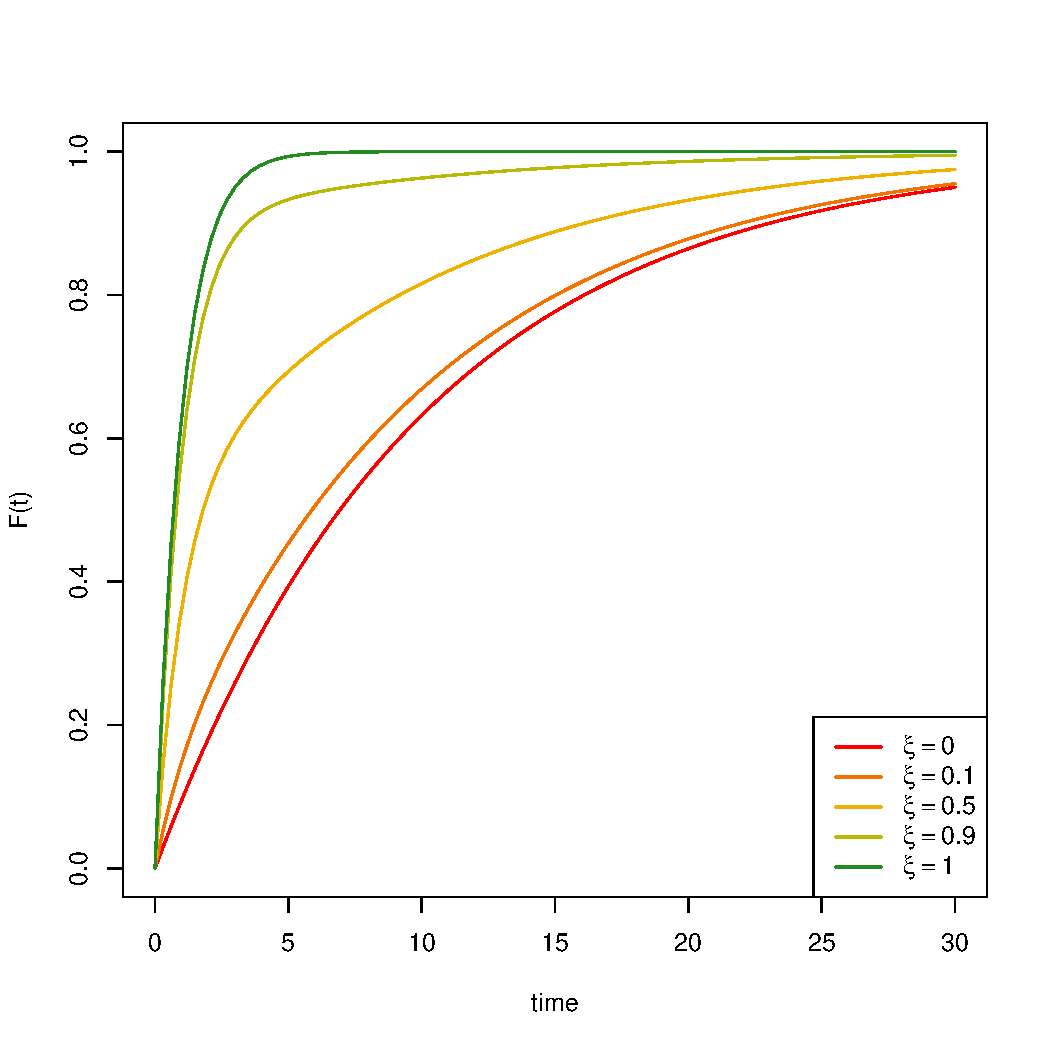
\includegraphics[width = .6\textwidth]{f_5_2_b.pdf}
	\item[(c)] 	\ \\ 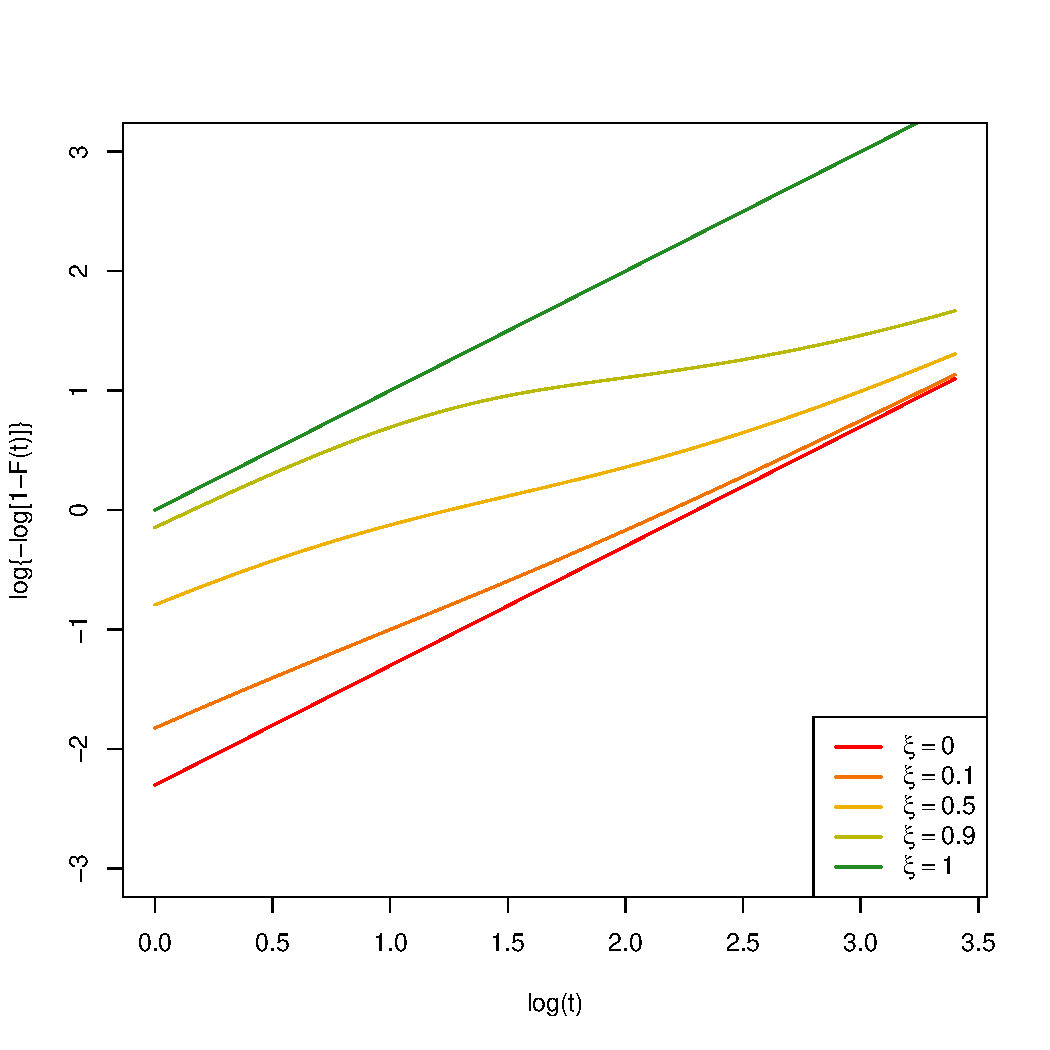
\includegraphics[width = .6\textwidth]{f_5_2_c.pdf}\\
			The pure exponential distributions, as $\xi = 0$ or $1$, are straight lines. Also, the mixture distributions are curves between the two straight lines.
	\item[(d)] 	\ \\ 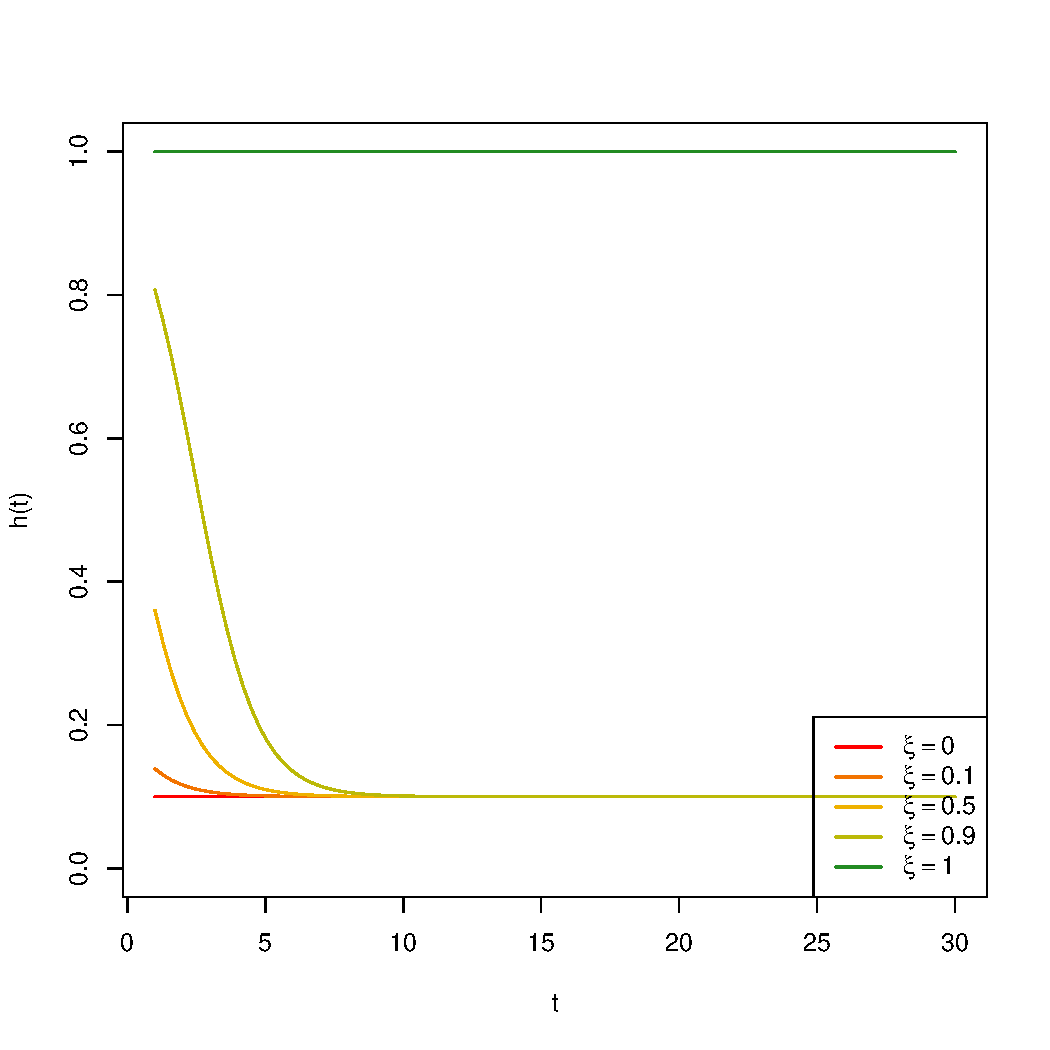
\includegraphics[width = .6\textwidth]{f_5_2_d.pdf}
	\item[(e)] 
\end{itemize}

\newpage
%----------------------------------------------------------------------------------------
%	6.5
%----------------------------------------------------------------------------------------
6.5
\begin{itemize}
	\item[(a)] \ \\ 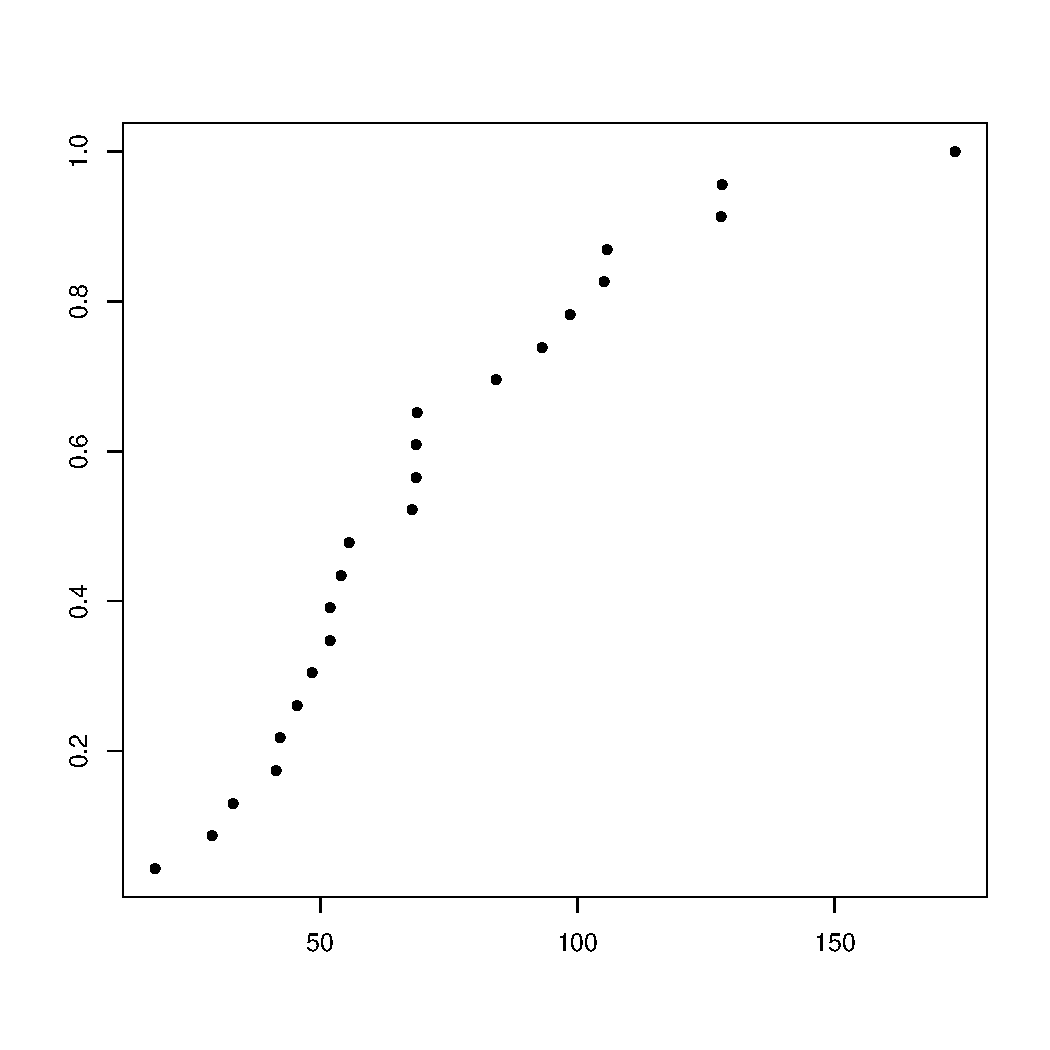
\includegraphics[width = .6\textwidth]{f_6_5_a.pdf}
	\item[(b)] \ \\ 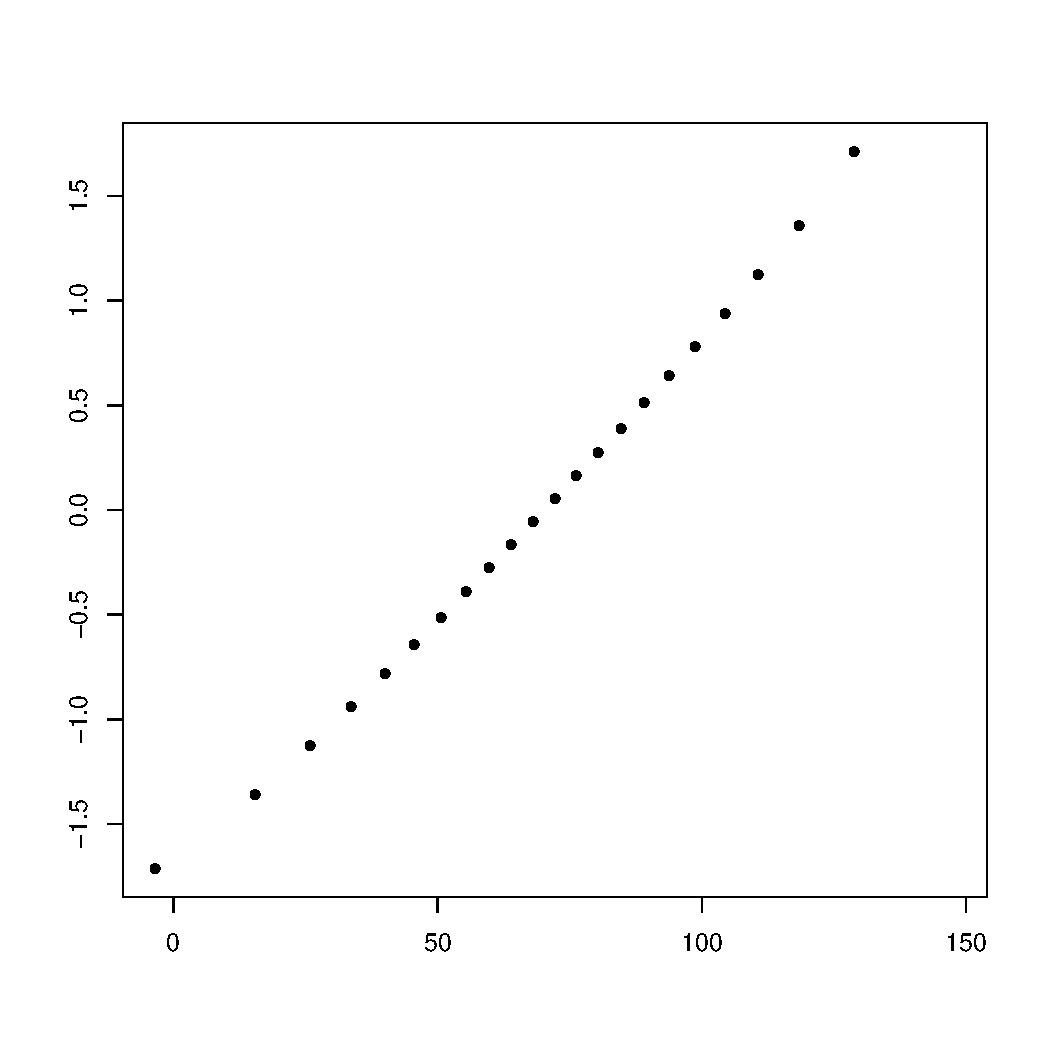
\includegraphics[width = .6\textwidth]{f_6_5_b.pdf}
	\item[(c)] \ \\ 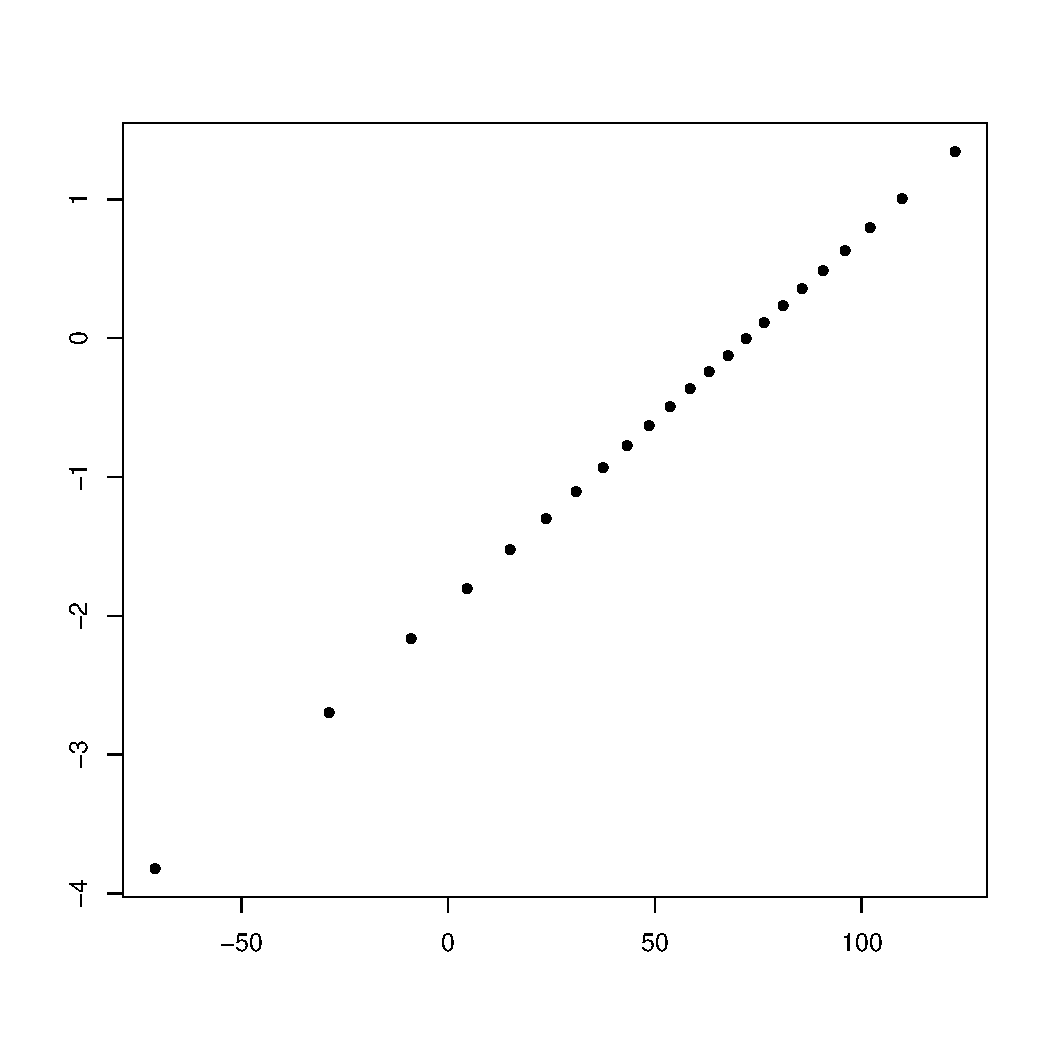
\includegraphics[width = .6\textwidth]{f_6_5_c.pdf}
	\item[(d)] This data fit log-normal distribution the most.
\end{itemize}

%----------------------------------------------------------------------------------------

\end{document} \\